\subsection{完成范围与计算核验}

本轮576条预锁记录中完成576条，失败/未决0条；独立背景72个，每例24个。两种响应律配对，四策略共享路径。不同观察360份，重复零计划不增加独立分母。

AC收敛55296个时点；设备约束违反0条、电压越限0条。新拟合与新WZZT搜索均为零。5项新增测试（含24组独立积分/梯度比较与已知可行的硬概率降费分支）和原12项测试通过；独立重放25240项通过。

\subsection{规划概率、独立核验与费用}

\begin{table}[ht]\centering\small\caption{同一4096点核验旧、新报价；费用为场景元/日}

\begin{tabular}{lrrrrr}\toprule 算例&规划概率&旧价核验&新价核验&旧费&新费\\\midrule

paper15&92.87\%&92.29\%&93.36\%&53.38&88.21\\

flynn16&36.94\%&34.16\%&36.12\%&72.20&92.18\\

pengwah18&0.00\%&0.00\%&0.00\%&0.00&0.00\\

\bottomrule\end{tabular}\end{table}

3个有历史争议条件中，本轮找到95\%规划可行报价0/3。pengwah是旧批事后已正确的零收益对照，但历史仍有争议，不能按真值跳过规划。未达标报价仅供诊断，不能据其称最小费用问题已解。独立核验不回流选价。

paper15独立核验标准误为0.245个百分点；工作分布下的Hoeffding单侧95\%下界为91.45\%。四阶段依次为均值初值、尾部初值、旧价启动和另一启动；停止状态依次为：迭代上限、时间上限、迭代上限、函数下降收敛。

flynn16独立核验标准误为0.478个百分点；工作分布下的Hoeffding单侧95\%下界为34.21\%。四阶段依次为均值初值、尾部初值、旧价启动和另一启动；停止状态依次为：迭代上限、时间上限、迭代上限、迭代上限。

pengwah18独立核验标准误为0.000个百分点；工作分布下的Hoeffding单侧95\%下界为0.00\%。四阶段依次为均值初值、尾部初值、旧价启动和另一启动；停止状态依次为：迭代上限、时间上限、投影梯度收敛、投影梯度收敛（概率仍为零）。

\subsection{实际AC后的完整恢复与错漏}

表中恢复的分母均为24，错漏为24日完整错漏总和。旧价与新价费用不同；同费比较只在新价与轮换之间成立。

\begin{table}[ht]\centering\small\caption{主响应及失配响应；所有失败保留}

\begin{tabular}{llrrrr}\toprule 算例&策略&主恢复&主错漏&失配恢复&失配错漏\\\midrule

paper15&无奖励&3/24&21&3/24&21\\

paper15&同费轮换&3/24&21&3/24&21\\

paper15&旧诊断价&20/24&4&20/24&4\\

paper15&新诊断价&21/24&3&20/24&4\\

\midrule

flynn16&无奖励&0/24&24&0/24&24\\

flynn16&同费轮换&0/24&24&0/24&24\\

flynn16&旧诊断价&0/24&24&0/24&24\\

flynn16&新诊断价&0/24&24&0/24&24\\

\midrule

pengwah18&无奖励&24/24&0&24/24&0\\

pengwah18&同费轮换&24/24&0&24/24&0\\

pengwah18&旧诊断价&24/24&0&24/24&0\\

pengwah18&新诊断价&24/24&0&24/24&0\\

\midrule

\bottomrule\end{tabular}\end{table}

\begin{figure}[p]\centering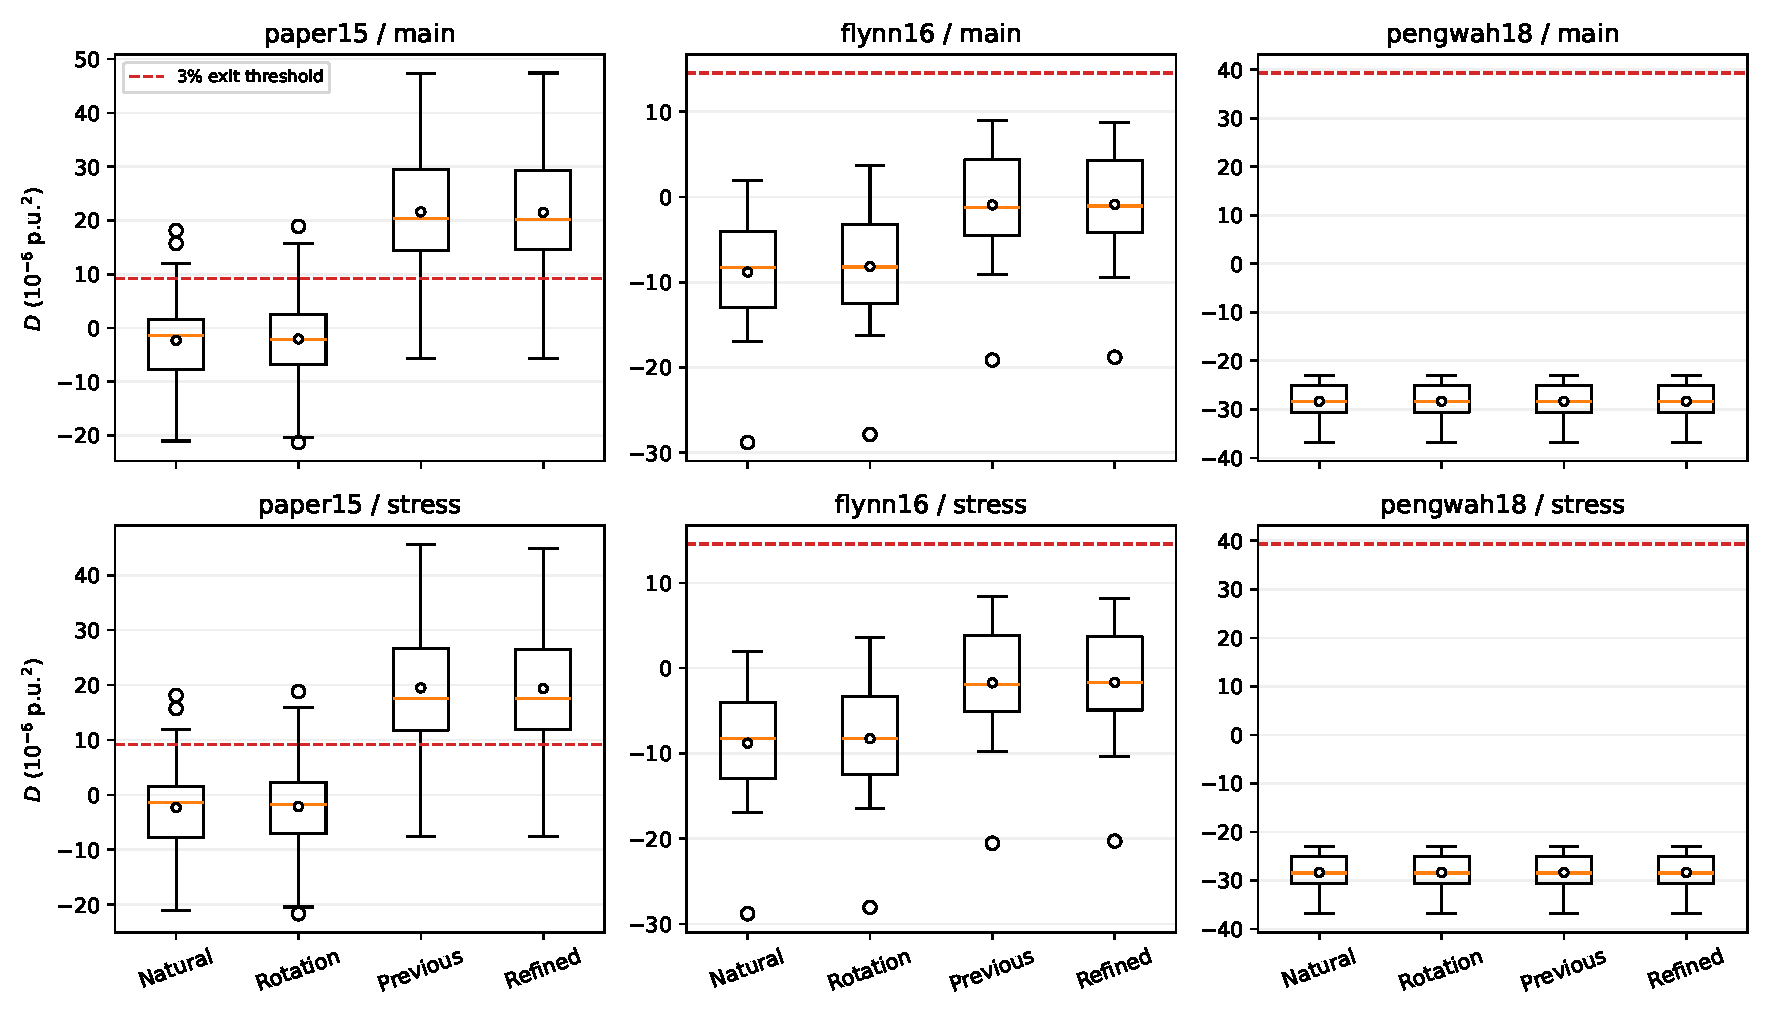
\includegraphics[width=\textwidth]{figures/loss_thresholds.pdf}\caption{冻结报价在独立AC路径上的实际损失差与原3\%排除阈值。箱线为24日结果；圆点表示均值，红线为历史阈值。显示指标是否足以触发选模，不能单独代表真实恢复。}\end{figure}\FloatBarrier

paper15主响应新价/旧价/轮换的实际绝对调节分别为158.61/95.80/201.14 kWh/日；新价平均净调节0.19 kWh/日。新价$D$均值21.505、最小-5.723，阈值9.179（微标幺平方）。

flynn16主响应新价/旧价/轮换的实际绝对调节分别为142.92/116.92/186.02 kWh/日；新价平均净调节-0.92 kWh/日。新价$D$均值-0.867、最小-18.791，阈值14.543（微标幺平方）。

pengwah18主响应新价/旧价/轮换的实际绝对调节分别为0.00/0.00/0.00 kWh/日；新价平均净调节0.00 kWh/日。新价$D$均值-28.351、最小-36.858，阈值39.314（微标幺平方）。

结果需按代价与可行性共同判断：若新价未达95\%、费用增加而实际恢复相同，就不将其作为已验证优于旧价的方法。保留旧价作为对照，下一步应针对参考预测与局部搜索瓶颈收口分析，不能用提高资源或降低选择阈值补出成功。
\subsection{本轮改进的判定}

paper15的新报价相对同费轮换，主响应18条改善、6条相同、0条变差；失配响应17条改善、7条相同、0条变差。新价的实际调节总量低于轮换，因此收益不能仅用“调节更多”解释。原始候选和冻结收缩输出在全部576条记录中错漏一致，改善保留到最终输出。

但相对旧报价，新价主响应仅1条改善、23条相同，失配响应24条全同，日费增加约65.24\%。独立工作概率仅由92.289\%增至93.359\%。flynn的工作概率由34.164\%增至36.123\%，实际仍未恢复。因而本轮没有支持将更贵新价作为默认替代方案，也没有解决95\%规划可行化。

纸面上的尾部初值并非本批收益的唯一解释：paper15最终最好点来自旧价启动的原概率搜索；flynn来自另一启动，但没有实际纠错增益。外层样本数和迭代量也同时改变，因此未作独立消融前，不将增益归因于尾部初始化。

下一步应保留较便宜旧价作为已验证对照，优先核查预测参考残差在新日AC下的失配来源，以及当前资源下阈值是否可达。三个训练日秩至多2的工作分布是具体缺口；继续增加局部迭代不能替代这一核查。本报告保留全部不达标和零收益情况，不以改变3\%、噪声或库存获得正结果。
